\documentclass[a4paper,10pt,american]{article}
\usepackage[a4paper,margin=1.2in]{geometry}
\usepackage{amsmath,amssymb,amsfonts,mathrsfs,accents} %important math packages
\usepackage{enumerate} % package for making different lists
\usepackage[T1]{fontenc} % Encoding of fonts
\usepackage{lmodern} % Latin modern font - needed for fontenc
\usepackage[utf8]{inputenc} % Encoding of input text
\usepackage[kerning]{microtype} % Better looking text
\usepackage[babel]{csquotes} % Better looking quotes
\usepackage{booktabs} % Better looking tables
\usepackage{babel} % Language control, for hyphenation etc
\usepackage{amsthm} % Package for theorem and definition enviroments
\usepackage[normalem]{ulem}
\usepackage{graphicx}
\usepackage{pgfplots}
\usepackage{tabularx}
\newcolumntype{C}{>{\centering\arraybackslash}X}
\usepackage{caption}
\usepackage{hyperref}
\usepackage{float}
\usepackage{tikz}
\usetikzlibrary{calc}
\usetikzlibrary{arrows}
\usepackage{pgfplots}
\pgfplotsset{compat=1.12}
\usetikzlibrary{patterns}
\usepgfplotslibrary{fillbetween}
\usepackage{listings}
\def \p{\par
\vspace{10pt}}

\def \sp{\par
\vspace{4pt}}

\setlength{\parindent}{0pt}
\newcommand{\ubar}[1]{\text{\b{$#1$}}}

% define command for convenience
\newcommand{\reals}{\mathbb{R}}

\title{Empirical Asset Pricing \\Assignment 2}
\author{Morteza Aghajanzadeh\thanks{Department of Finance, Stockholm School of Economics. Email: morteza.aghajanzadeh@phdstudent.hhs.se} }

\date{\today}
\setlength\parindent{0pt}

\newcommand\scalemath[2]{\scalebox{#1}{\mbox{\ensuremath{\displaystyle #2}}}}


\begin{document}
	\maketitle


\section*{Question 1}
\begin{enumerate}[(a)]

  \item Here are the moments and the correlation of the moments:
  \begin{table}[htbp!]
    \centering
    \caption{Table of the moments}
    \label{tab:1a}
    \begin{tabular}{lrrrr}
\toprule
 & $\Delta c$ & $r_{m,t}$ & $r_{f,t}$ & $r_{e,t}$ \\
\midrule
$\mu$ & 0.018 & 0.060 & 0.005 & 0.054 \\
$\sigma$ & 0.021 & 0.197 & 0.029 & 0.197 \\
$\rho_1$ & 0.504 & -0.010 & 0.676 & 0.019 \\
\bottomrule
\end{tabular}

  \end{table}
  \begin{table}[htbp!]
    \centering
    \caption{Table of the correlation of the moments}
    \label{tab:1a_corr}
    \begin{tabular}{lrrrr}
\toprule
 & $\Delta c$ & $r_{m,t}$ & $r_{f,t}$ & $r_{e,t}$ \\
\midrule
$\Delta c$ & 0.000 & 0.000 & -0.000 & 0.001 \\
$r_{m,t}$ & 0.000 & 0.039 & 0.000 & 0.038 \\
$r_{f,t}$ & -0.000 & 0.000 & 0.001 & -0.000 \\
$r_{e,t}$ & 0.001 & 0.038 & -0.000 & 0.039 \\
\bottomrule
\end{tabular}

  \end{table}
  \item Given the moments and correlation that we calculate in the previous question, we can use the equation (2) in the question to estimate the parameters. The equation is as follows:
  \begin{gather*}
    \mathbb{E}[r_{i,t}-r_{f,t}] + \frac{\sigma^2_i}{2} = \gamma \sigma_{ic} \\
    \Rightarrow \gamma = \frac{\mathbb{E}[r_{i,t}-r_{f,t}] + \frac{\sigma^2_i}{2}}{\sigma_{ic}} 
  \end{gather*}
  \begin{enumerate}[i.]
   \item  If we use the sample moments for calculating the parameters, we get that $\gamma_1 = 1.358$.
   \item If we assume that the correlation between
   excess returns on stocks and consumption growth equals one, we get that $\gamma_2 = 16.585$.
  \end{enumerate}
  The outcomes differ, as expected, given our assumption of perfect correlation between stock returns and consumption growth in the second scenario. This assumption results in a significantly high value for the risk aversion parameter $\gamma$. The strong correlation implies that stock returns are highly responsive to changes in consumption growth, increasing their riskiness and consequently elevating the value of $\gamma$.
  \item Now we need to use the estimated parameters to estimate the time discount factor $\delta$. We can use the equation (3) in the question to estimate the time discount factor. The equation is as follows:
  \begin{gather*}
    r_{f,t} = - \ln(\delta) + \gamma\mathbb{E}[\Delta c_t ] - \frac{\gamma^2 \sigma_c^2}{2} 
  \end{gather*}
  as we write the equation for the average of the risk-free rate, we get:
  \begin{gather*}
    \mathbb{E}[r_{f,t}] = - \ln(\delta) + \gamma\mathbb{E}[\Delta c_t ] - \frac{\gamma^2 \sigma_c^2}{2}\\
    \Rightarrow \delta = \exp(- \mathbb{E}[r_{f,t}] + \gamma\mathbb{E}[\Delta c_t ] - \frac{\gamma^2 \sigma_c^2}{2} )
  \end{gather*}
  which for given moments and different values of $\gamma$ we get the following values for $\delta$:
  \begin{enumerate}[i.]
    \item Base on $\gamma_1$, we get that $\delta_1 = 1.019$ and time preference rate of $ -0.019$.
    \item Base on $\gamma_2$, we get that $\delta_2 = 1.267$ and time preference rate of $-0.237$.
  \end{enumerate}

  \item Now we need to use the GMM estimator to estimate the parameters in order to have standard errors for the estimators. Let's define the variables as follows:
  \begin{equation*}
    \begin{aligned}
      f(v_t,\theta) = & \begin{bmatrix}
        \Delta c_t - \mu_c \\
        r_{m,t} - \mu_m \\
        r_{m,t} - r_{f,t} + \frac{1}{2} (r_{m,t} - \mu_m)^2 - \gamma (r_{m,t} - \mu_m)(\Delta c_t - \mu_c) \\
        r_{f,t} + \ln(\delta) -\gamma\Delta c_t +  \frac{1}{2}\gamma^2 (\Delta c_t - \mu_c)^2 \\
      \end{bmatrix} & , \quad 
      \theta = & \begin{bmatrix}
        \mu_c \\
        \mu_m \\
        \gamma \\
        \delta \\
      \end{bmatrix}  \\
      g_T(\theta) = & \quad \frac{1}{T} \sum_{t=1}^T f(v_t,\theta) & \\
    \end{aligned}
    \end{equation*}
    As we can see, the system is exactly identified, since the number of parameters is equal to the number of moments. So, we can use the GMM estimator to estimate the parameters.
    
      \begin{gather*}
        g_T(\theta) = 0\\
        \Rightarrow\frac{1}{T} \sum_{t=1}^T f(v_t,\theta) = 0\\
        \Rightarrow\frac{1}{T} \sum_{t=1}^T \begin{bmatrix}
          \Delta c_t - \mu_c \\
          r_{m,t} - \mu_m \\
          r_{m,t} - r_{f,t} + \frac{1}{2} (r_{m,t} - \mu_m)^2 - \gamma (r_{m,t} - \mu_m)(\Delta c_t - \mu_c) \\
          r_{f,t} + \ln(\delta) -\gamma\Delta c_t +  \frac{1}{2}\gamma^2 (\Delta c_t - \mu_c)^2 \\
        \end{bmatrix} = 0 
      \end{gather*}
        \begin{gather*}
        \Rightarrow \begin{bmatrix}
          \frac{1}{T} \sum_{t=1}^T \Delta c_t - \mu_c \\
          \frac{1}{T} \sum_{t=1}^T r_{m,t} - \mu_m \\
          \frac{1}{T} \sum_{t=1}^T r_{m,t} - r_{f,t} + \frac{1}{2} (r_{m,t} - \mu_m)^2 - \gamma (r_{m,t} - \mu_m)(\Delta c_t - \mu_c) \\
          \frac{1}{T} \sum_{t=1}^T r_{f,t} + \ln(\delta) -\gamma\Delta c_t +  \frac{1}{2}\gamma^2 (\Delta c_t - \mu_c)^2 \\
        \end{bmatrix} = 0 
      \end{gather*}
      \begin{equation*}
        \Rightarrow \begin{bmatrix}
          \mathbb{E} [\Delta c_t] - \mu_c \\
          \mathbb{E} [r_{m,t}] - \mu_m \\
          \mathbb{E} [r_{m,t}- r_{f,t}]  + \frac{1}{2}\mathbb{E} [ (r_{m,t} - \mu_m)^2] - \gamma \mathbb{E} [(r_{m,t} - \mu_m)(\Delta c_t - \mu_c)] \\
          \mathbb{E} [r_{f,t}] + \ln(\delta) -\gamma\mathbb{E} [\Delta c_t] +  \frac{1}{2}\gamma^2 \mathbb{E} [(\Delta c_t - \mu_c)^2] \\
        \end{bmatrix} = 0
      \end{equation*}
      \begin{equation*}
        \Rightarrow \begin{bmatrix}
          \mu_c - \mathbb{E} [\Delta c_t] \\
          \mu_m - \mathbb{E} [r_{m,t}] \\
          \gamma - \frac{\mathbb{E} [r_{m,t}- r_{f,t}] + \hat{\sigma}_m^2/2}{\hat{\sigma}_{mc} } \\
          \delta - exp(- \mathbb{E} [r_{f,t}] + \gamma\mathbb{E} [\Delta c_t] - \frac{1}{2}\gamma^2 \sigma_c^2 )  \\
        \end{bmatrix} = 0
      \end{equation*}
      \begin{equation*}
        \rightarrow  \theta = \begin{bmatrix}
          \mathbb{E} [\Delta c_t] \\
          \mathbb{E} [r_{m,t}] \\
          \frac{\mathbb{E} [r_{m,t}- r_{f,t}] + \hat{\sigma}_m^2/2}{\hat{\sigma}_{mc} } \\
          exp(- \mathbb{E} [r_{f,t}] + \gamma\mathbb{E} [\Delta c_t] - \frac{1}{2}\gamma^2 \sigma_c^2 )  \\
        \end{bmatrix}
      \end{equation*}
      where $\hat{\sigma}_m^2$ is the sample variance of $r_{m,t}$ and $\hat{\sigma}_{mc}$ is the sample covariance of $r_{m,t}$ and $\Delta c_t$.

      As we can see it is the same method as we used for estimating in the first method of previous question. The only difference is that now we can estimate the variance of the estimator by using the equation for the variance of the GMM estimator. The Newey-West adjusted variance of the estimator is as follows:    
      \begin{equation*}
        \hat{S}_T = \frac{1}{T} \sum_{t=1}^T f(v_t,\hat{\theta})f(v_t,\hat{\theta}) + \frac{1}{2}(\hat{\Gamma}_1 + \hat{\Gamma}_1')
      \end{equation*}
      where $\hat{\theta}$ is the estimated parameter vector. 

      Calculate the variance of the estimator analytically is a bit more complicated, but it is possible. I will only drive the variance of the estimator numerically. 
      \begin{table}[htbp!]
        \centering
        \caption{Newey-West adjusted variance of the estimator}
        \label{tab:1d}
        \begin{tabular}{lrrrr}
\toprule
{} &  \$\textbackslash mu\_c\$ &  \$\textbackslash mu\_m\$ &  \$\textbackslash gamma\$ &  \$\textbackslash delta\$ \\
\midrule
\$\textbackslash mu\_c\$  &   0.0007 &   0.0013 &    0.0081 &   -0.4310 \\
\$\textbackslash mu\_m\$  &   0.0013 &   0.0379 &    0.1080 &   -0.9938 \\
\$\textbackslash gamma\$ &   0.0081 &   0.1080 &    1.0622 &   -7.9041 \\
\$\textbackslash delta\$ &  -0.4310 &  -0.9938 &   -7.9041 &  507.0663 \\
\bottomrule
\end{tabular}

      \end{table}

      \item Now we change the target moments to be the following:
      \begin{equation*}
        \begin{aligned}
          f(v_t,\theta) = & \begin{bmatrix}
            \exp(\ln(\delta) - \gamma\Delta c_t + r_{m,t})-1 \\
            \exp(\ln(\delta) - \gamma\Delta c_t + r_{f,t})-1
          \end{bmatrix} & , \quad 
          \theta = & \begin{bmatrix}
            \gamma \\
            \delta \\
          \end{bmatrix}  \\
          g_T(\theta) = & \quad \frac{1}{T} \sum_{t=1}^T f(v_t,\theta) & \\
        \end{aligned}
        \end{equation*}
        again the system is exactly identified, since the number of parameters is equal to the number of moments. So, we can use the GMM estimator to estimate the parameters.
        \begin{gather*}
          g_T(\theta) = 0\\
          \Rightarrow\frac{1}{T} \sum_{t=1}^T f(v_t,\theta) = 0\\
          \Rightarrow\frac{1}{T} \sum_{t=1}^T \begin{bmatrix}
            \exp(\ln(\delta) - \gamma\Delta c_t + r_{m,t})-1 \\
            \exp(\ln(\delta) - \gamma\Delta c_t + r_{f,t})-1
          \end{bmatrix} = 0\\
          \Rightarrow \begin{bmatrix}
            \frac{1}{T} \sum_{t=1}^T \exp(\ln(\delta) - \gamma\Delta c_t + r_{m,t})-1 \\
            \frac{1}{T} \sum_{t=1}^T \exp(\ln(\delta) - \gamma\Delta c_t + r_{f,t})-1
          \end{bmatrix} = 0\\
          \Rightarrow \begin{bmatrix}
            \mathbb{E} [\exp(\ln(\delta) - \gamma\Delta c_t + r_{m,t})]-1 \\
            \mathbb{E} [\exp(\ln(\delta) - \gamma\Delta c_t + r_{f,t})]-1
          \end{bmatrix} = 0
        \end{gather*}

        As our target moments are non-linear, we can not use the same method as we used for the linear moments. So we need to use the numerical optimization methods to estimate the parameters. 

        Here we use the FOC of the GMM estimator which is as follows:
        \begin{equation*}
          g_T(\theta) = 0
        \end{equation*}
        and in the optimization I try to minimize the loss function which is quadratic one.
        \begin{lstlisting}[language=Python, caption= Python code for defining the moments and the loss function for the non-linear moments, label={pcode:1e}, escapechar=|, frame=single, basicstyle=\small, showstringspaces=false, captionpos=b, breaklines=true, showspaces=false, showtabs=false, keywordstyle=\color{blue}, commentstyle=\color{gray}]
          def f_v(theta,x):
            gamma = theta[0]
            delta = theta[1]
            x_c = x[0]
            x_m = x[1]
            x_e = x[2]
            r_f = x_m - x_e
            f = np.array([
                np.exp(np.log(delta) - gamma * x_c + x_m) - 1,
                np.exp(np.log(delta) - gamma * x_c + r_f) - 1,
                ]).reshape(len(theta),1)
            return f

          def FOC(theta,x):
              return sum([f_v(theta,i) for i in x])/len(x)

          def loss(theta,x):
              return (FOC(theta,x).T @ FOC(theta,x))[0][0]
    \end{lstlisting}
    
    \begin{table}[htbp!]
      \centering
      \caption{Estimation of the parameters for the non-linear moments}
      \label{tab:1e}
      \begin{tabular}{lrr}
\toprule
 & $\gamma$ & $\delta$ \\
\midrule
$\hat{\theta}$ & 44.69 & 0.91 \\
\bottomrule
\end{tabular}

    \end{table}
    \begin{table}[htbp!]
      \centering
      \caption{Newey-West adjusted variance of the estimator for the non-linear moments}
      \label{tab:1e_sd}
      \begin{tabular}{lrr}
\toprule
 & $\gamma$ & $\delta$ \\
\midrule
$\gamma$ & 15.6633 & 16.3156 \\
$\delta$ & 16.3156 & 17.1580 \\
\bottomrule
\end{tabular}

    \end{table}
\end{enumerate}

\section*{Question 3}
I just wrote a function that create the portfolios and calculate the portfolio return based on "Equal" and "Market" weighting. The function is shown in the code \ref{pcode:3a}. The function takes the following inputs:
\begin{itemize}
    \item \textbf{df}: The dataframe that contains the data
    \item \textbf{sorting\_car}: The variable that will be used to sort the stocks
    \item \textbf{number\_of\_portfolios}: The number of portfolios that will be created
    \item \textbf{weighting}: The type of weighting that will be used to calculate the portfolio return. The default is "Equal" weighting.
\end{itemize}

\begin{lstlisting}[language=Python, caption= Python function to create portfolios, label={pcode:3a}, escapechar=|, frame=single, basicstyle=\small, showstringspaces=false, captionpos=b, breaklines=true, showspaces=false, showtabs=false, keywordstyle=\color{blue}, commentstyle=\color{gray}]
    def get_portfolios(df, sorting_car, number_of_portfolios,weighting = 'Equal'):
    portfoli_df = df.dropna(subset=[sorting_car])[
        ['t', 'permno', sorting_car, 'me', 'ret']
    ].copy()
    portfoli_df['portfolios'] = portfoli_df.groupby('t')[sorting_car].transform(lambda x: pd.qcut(x, number_of_portfolios, labels=False)) 
    portfoli_df['portfolios'] = portfoli_df['portfolios'] + 1   # The highest value is the highest portfolio
    if weighting == 'market':
        portfoli_df['weight'] = portfoli_df.groupby(['t','portfolios'])['me'].transform(lambda x: x/sum(x))
        portfoli_df['ret'] = portfoli_df['ret'] * portfoli_df['weight']
    elif weighting == 'Equal':
        portfoli_df['weight'] = portfoli_df.groupby(['t','portfolios'])['me'].transform(lambda x: 1/len(x))
        portfoli_df['ret'] = portfoli_df['ret'] * portfoli_df['weight']
    return portfoli_df.groupby(['t','portfolios']).ret.sum().unstack().reset_index().rename(columns = {"t":"month"})
\end{lstlisting}

\begin{enumerate}[(a)]
\item Here is the result of the function for the "Equal" weighting. (Figure \ref{fig:3a}) As we can see, at the beginning of the sample, all the portfolios have the same return. However, as time goes by, the return of the portfolios start to diverge. At the end of the sample, the cumulative return of the highest portfolio is much lower than the lowest portfolio. 
\begin{figure}[htbp!]
    \centering
    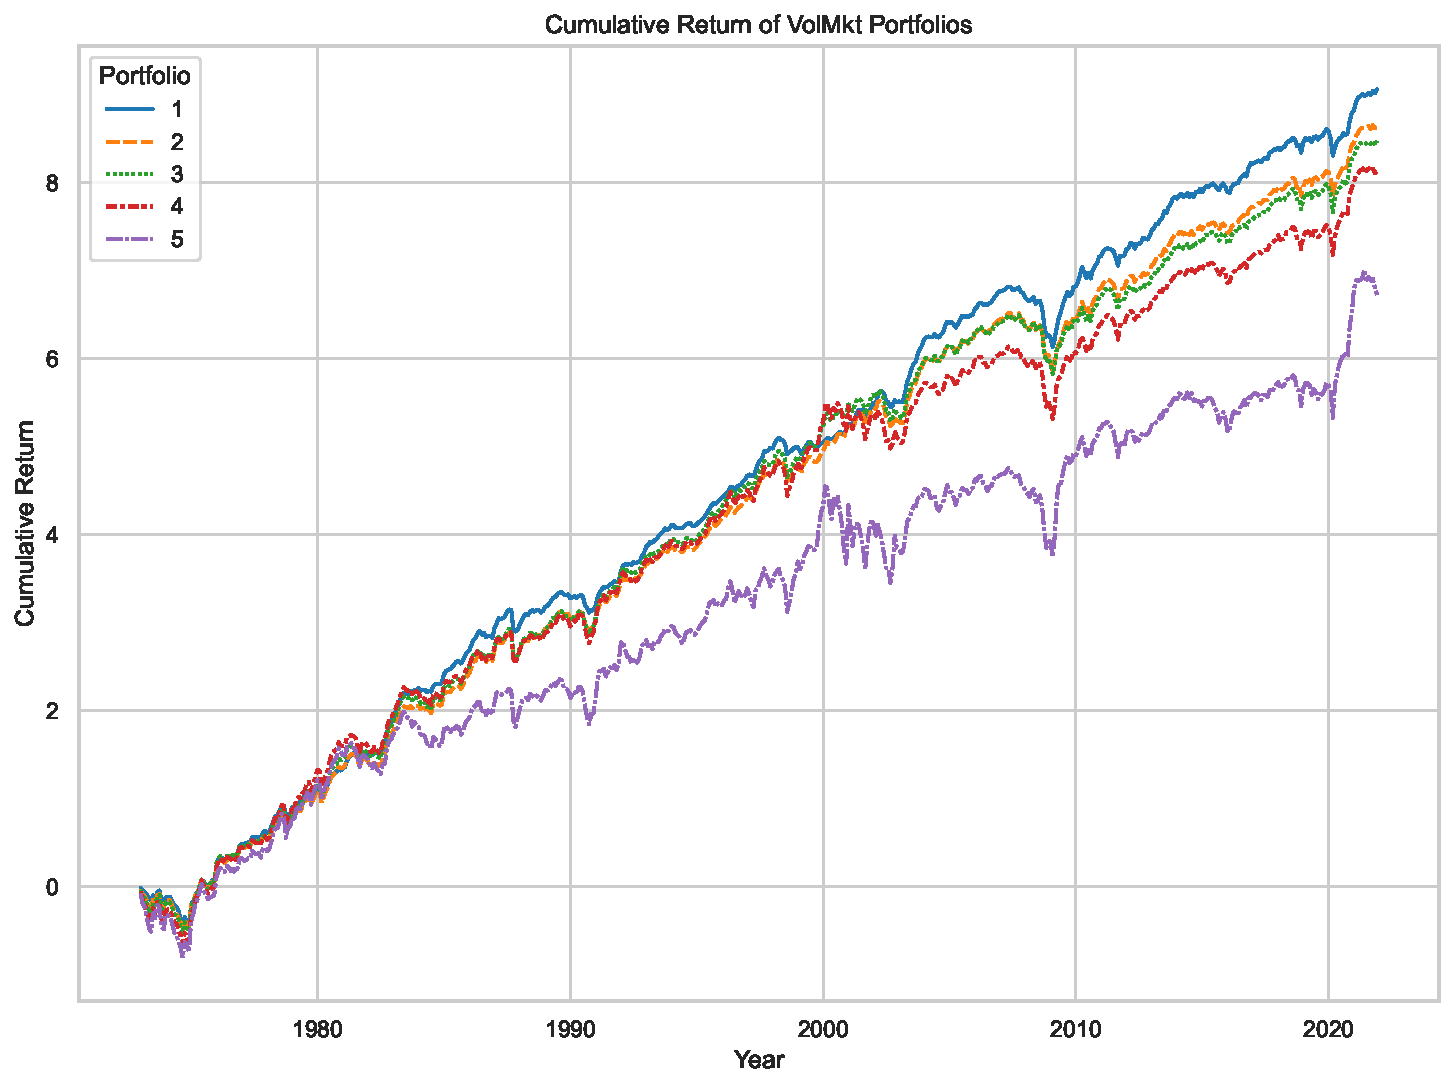
\includegraphics[width=0.6\textwidth]{Out/3_1.pdf}
    \caption{Time series of the average returns of the portfolios based on the "Equal" weighting.}
    \label{fig:3a}
\end{figure}

\item Here is the result of the function for the "Market" weighting. (Figure \ref{fig:3b}) As we can see, the market weighting does not have the same pattern as the "Equal" weighting. The return of the portfolios are stay close to each other and do not diverge as much as the "Equal" weighting. In fact, the cumulative return of the highest portfolio is higher than the lowest portfolio which is the opposite of the "Equal" weighting. I report the average return of the portfolios in the table \ref{tab:3b}.
\begin{figure}
    \centering
    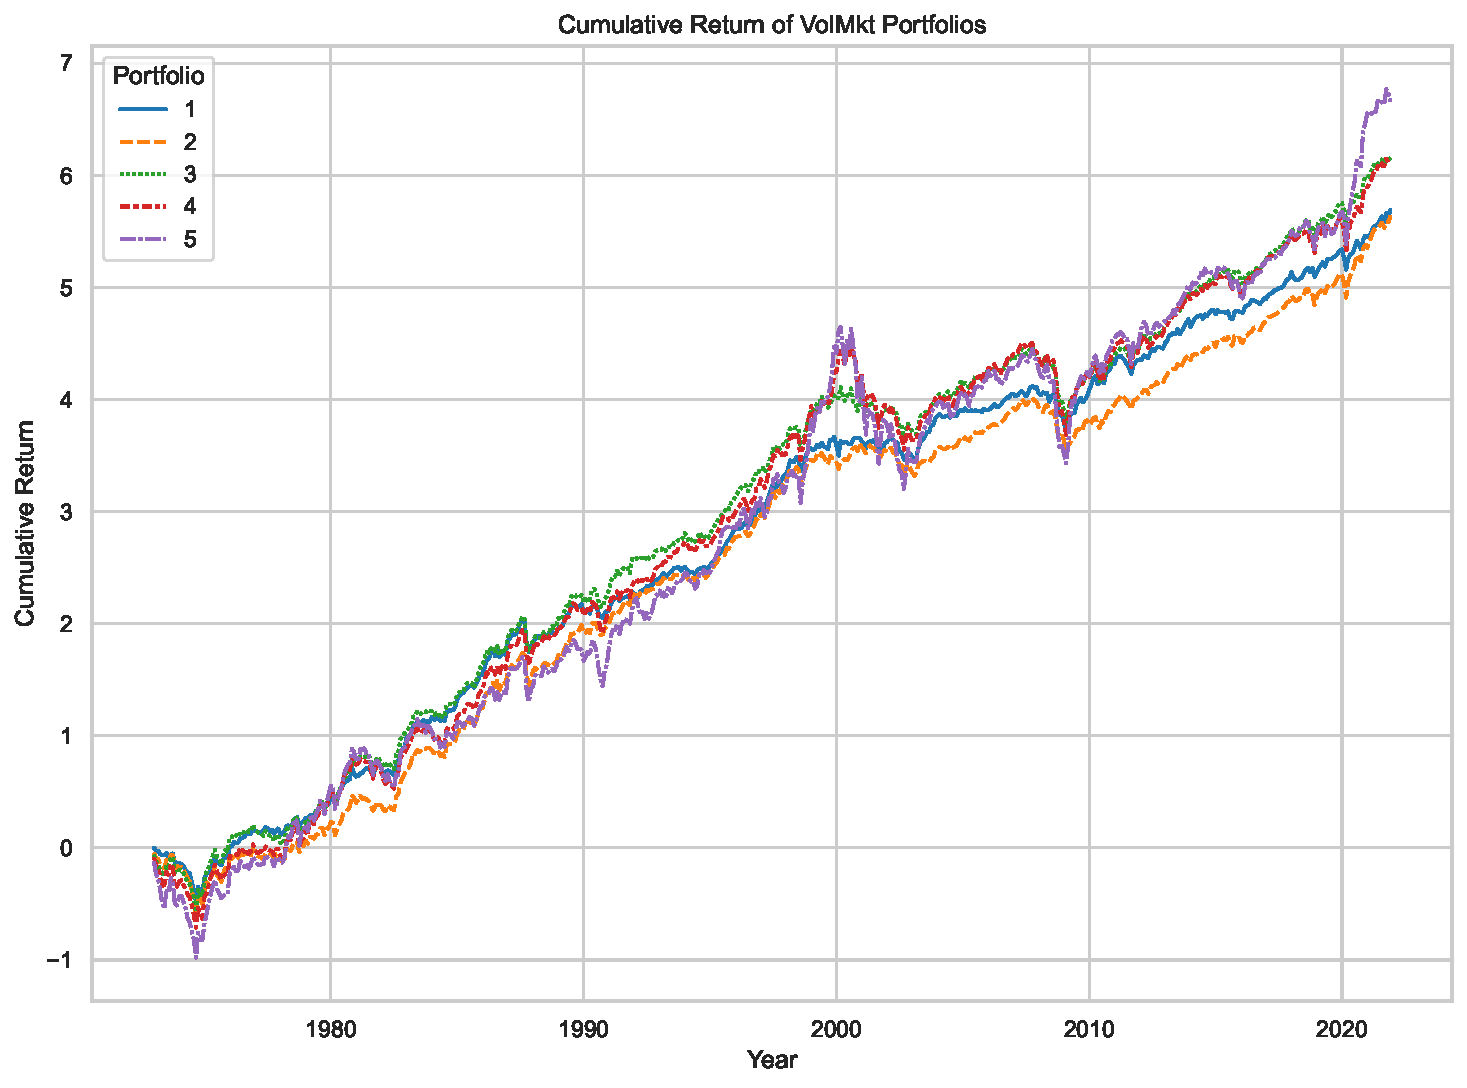
\includegraphics[width=0.6\textwidth]{Out/3_2.pdf}
    \caption{Time series of the average returns of the portfolios based on the "Market" weighting.}
    \label{fig:3b}
\end{figure}

\begin{table}[htbp!]
    \centering
    \caption{Average returns of the portfolios with different weighting}
    \label{tab:3b}
    \begin{tabular}{lrrrrr}
\toprule
portfolios &  Lowest &      2 &      3 &      4 &  Highest \\
\midrule
Equal Weighted  &  0.0154 & 0.0147 & 0.0144 & 0.0138 &   0.0114 \\
Market Weighted &  0.0097 & 0.0096 & 0.0105 & 0.0104 &   0.0113 \\
\bottomrule
\end{tabular}

\end{table}

\item Here we create the long-short portfolio. The long-short portfolio is created by taking the difference between the returns of the highest and the lowest portfolio. The result is shown in the figure \ref{fig:3c}. As we can see, the long-short portfolio has a positive return for the equal weighting and a negative return for the market weighting.

\begin{figure}[htbp!]
    \centering
    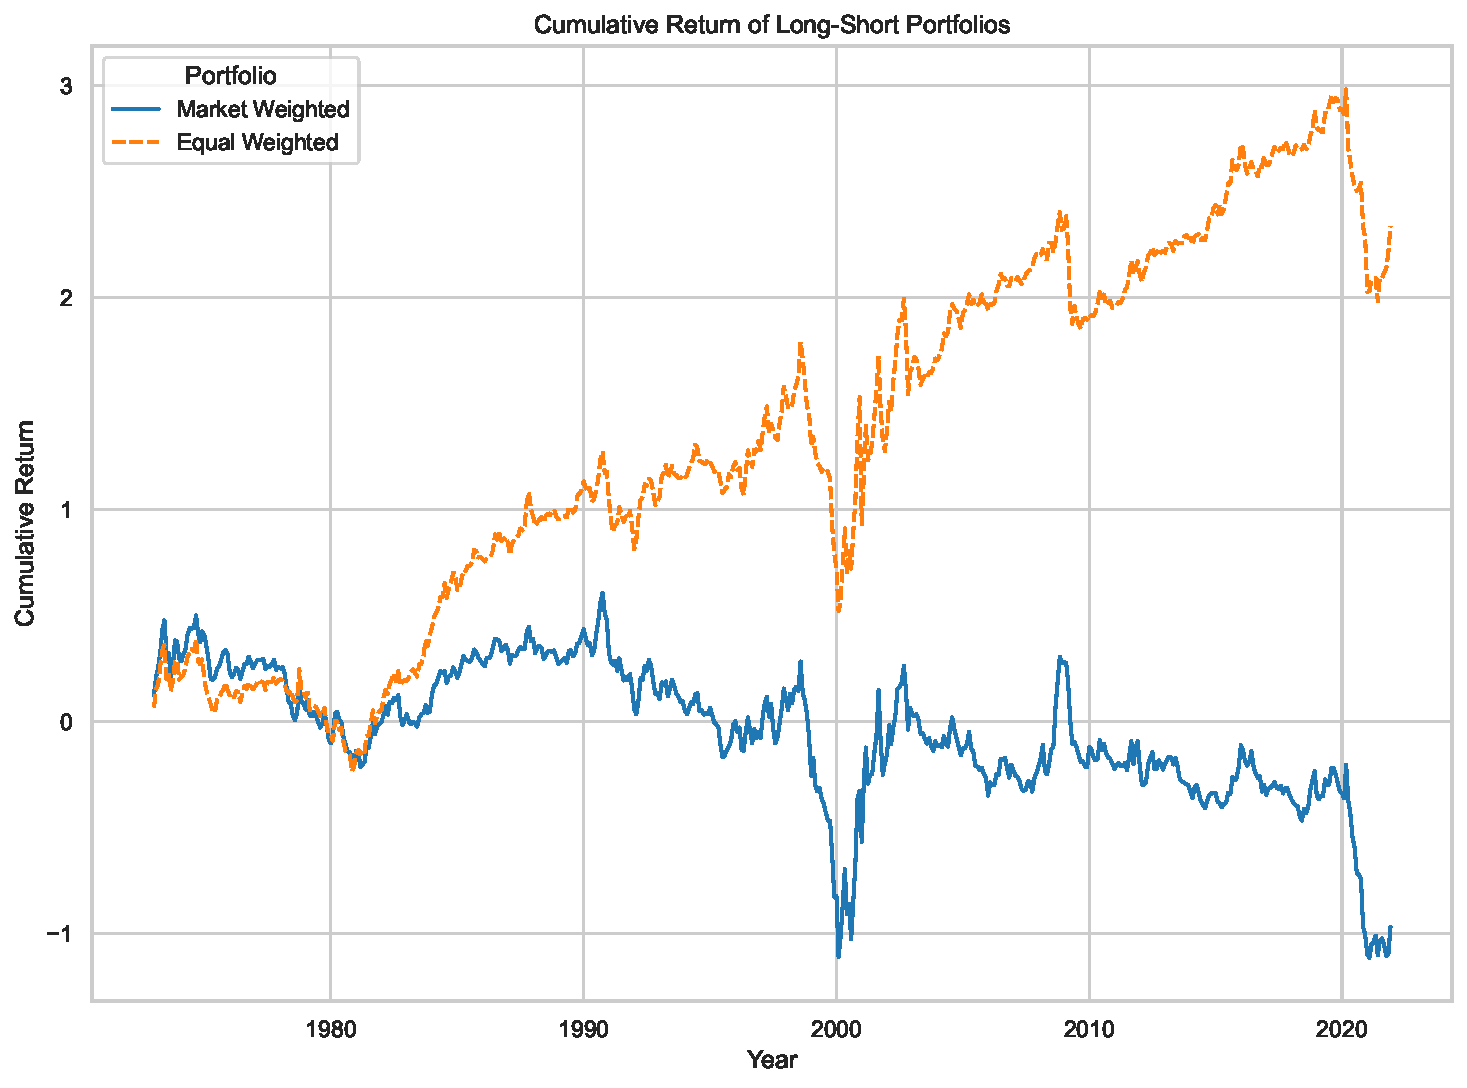
\includegraphics[width=0.6\textwidth]{Out/3_3.pdf}
    \caption{Time series of the average returns of the long-short portfolio.}
    \label{fig:3c}
\end{figure}

Now we can test the CAPM, Fama-French 3 factors and the Fama-French 5 factors, Carhart, and HXZ models. You can find the function that I write to test the null hypothesis that $\alpha_{LS} =0$. I will use the Newey-West standard errors to test the null hypothesis. The result of the test is shown in the table \ref{tab:3c}.


\begin{lstlisting}[language=Python, caption= Python function to run the test, label={pcode:3a}, escapechar=|, frame=single, basicstyle=\small, showstringspaces=false, captionpos=b, breaklines=true, showspaces=false, showtabs=false, keywordstyle=\color{blue}, commentstyle=\color{gray}]
    def time_series_regression(portfolios, factors, FactorModel):
    portfolios = portfolios.merge(factors, on='month', how='left')
    portfolios = portfolios.dropna()
    X = portfolios[FactorModel]
    X = sm.add_constant(X)
    Y = portfolios['long_short']
    model = sm.OLS(Y, X).fit(cov_type='HAC',cov_kwds={'maxlags':int(len(Y)**0.25)}) 
    pvalues = model.pvalues
    betas = model.params
    return [betas.iloc[0],pvalues.iloc[0]]
\end{lstlisting}

You can find the result of the test in the table \ref{tab:3c} for CAPM, Fama-French 3 factors, Fama-French 5 factors, Carhart, and HXZ models. 
\begin{table}[htbp!]
    \caption{$\alpha$ test for long-short portfolio with different models}
    \label{tab:3c}
    \begin{tabularx}{\linewidth}{CC}
        \caption*{Equal Weighted }
        \begin{tabular}{lcc}
\toprule
 & $\alpha$ & $Pvalue$ \\
\midrule
CAPM & 0.010 & 0.000 \\
FF3 & 0.008 & 0.000 \\
CAR & 0.003 & 0.167 \\
FF5 & 0.003 & 0.167 \\
HXZ & 0.000 & 0.944 \\
\bottomrule
\end{tabular}

        &
        \caption*{Market Weighted }
        \begin{tabular}{lcc}
\toprule
 & $\alpha$ & $Pvalue$ \\
\midrule
CAPM & 0.004 & 0.073 \\
FF3 & 0.002 & 0.267 \\
CAR & -0.000 & 0.790 \\
FF5 & -0.003 & 0.061 \\
HXZ & -0.004 & 0.036 \\
\bottomrule
\end{tabular}

    \end{tabularx}
\end{table}
\item 
Now we can test the long-short portfolio for in and out of sample. The result is shown in the table \ref{tab:3d1} for the equal weighting and in the table \ref{tab:3d2} for the market weighting. As we can see, the long-short portfolio has a positive return for the equal weighting and a negative return for the market weighting. The result is consistent with the previous result.
\begin{table}[htbp]
    \caption{$\alpha$ test long-short portfolio for in and out of sample with equal weighting}
    \label{tab:3d1}
    \begin{tabularx}{\linewidth}{CC}
        \caption*{Sample period }
        \begin{tabular}{lcc}
\toprule
 & $\alpha$ & $Pvalue$ \\
\midrule
CAPM & 0.010 & 0.000 \\
FF3 & 0.008 & 0.000 \\
CAR & 0.006 & 0.008 \\
FF5 & 0.005 & 0.016 \\
HXZ & 0.005 & 0.081 \\
\bottomrule
\end{tabular}

        &
        \caption*{Post-publication period}
        \begin{tabular}{lcc}
\toprule
 & $\alpha$ & $Pvalue$ \\
\midrule
CAPM & 0.012 & 0.002 \\
FF3 & 0.011 & 0.000 \\
CAR & 0.007 & 0.027 \\
FF5 & 0.005 & 0.132 \\
HXZ & 0.001 & 0.777 \\
\bottomrule
\end{tabular}

    \end{tabularx}
\end{table}

\begin{table}[htbp]
    \caption{$\alpha$ test long-short portfolio for in and out of sample with market weighting}
    \label{tab:3d2}
    \begin{tabularx}{\linewidth}{CC}
        \caption*{Sample period }
        \begin{tabular}{lcc}
\toprule
 & $\alpha$ & $Pvalue$ \\
\midrule
CAPM & 0.004 & 0.089 \\
FF3 & 0.002 & 0.346 \\
CAR & 0.000 & 0.911 \\
FF5 & -0.000 & 0.896 \\
HXZ & -0.001 & 0.821 \\
\bottomrule
\end{tabular}

        &
        \caption*{Post-publication period}
        \begin{tabular}{lcc}
\toprule
 & $\alpha$ & $Pvalue$ \\
\midrule
CAPM & 0.005 & 0.115 \\
FF3 & 0.004 & 0.056 \\
CAR & 0.002 & 0.286 \\
FF5 & -0.002 & 0.389 \\
HXZ & -0.003 & 0.198 \\
\bottomrule
\end{tabular}

    \end{tabularx}
\end{table}


\end{enumerate}

\section*{Question 4}
\begin{enumerate}[(a)]
    \item We predict the out-of-sample returns based on three different models:
    \begin{enumerate}[i.]
        \item Using dividend-price ratio:
            \begin{equation*}
                    \hat{R}_{t,DP}^e = \hat{\alpha} + \hat{\beta}_{t-1} dp_{t-1}  
            \end{equation*}
        \item Using all the variables from Dong et al. (2022):
            \begin{equation*}
                \hat{R}_{t,OLS}^e = \hat{\alpha} + \sum_{i=1}^{K}\hat{\beta}_{i,t-1} X_{i,t-1}
            \end{equation*}
        \item Using combination-mean forecast:
            \begin{equation*}
                \hat{R}_{t,CM}^e = \frac{1}{K}\sum_{i=1}^{K} \hat{R}_{t,i}^e
            \end{equation*}
            where, for each $i$,
            \begin{equation*}
                \hat{R}_{t,i}^e = \hat{\alpha}_i + \hat{\beta}_{i,t-1} dp_{t-1}
            \end{equation*}
    \end{enumerate}
    where $\hat{\alpha}$ and $\hat{\beta}$ are estimated using OLS regression for the in-sample data which is an expanding window from 1970/01 until the previous month of the out-of-sample period. The out-of-sample period is from 1985/01 until 2017/12. We compare each model using the out-of-sample $R^2$ which is defined as:
    \begin{equation*}
        R^2_{oc} = 1 - \frac{\sum_{t=1}^{T} (R_{t}^e - \hat{R}_{t}^e)^2}{\sum_{t=1}^{T} (R_{t}^e - \bar{R}_{t}^e)^2}
    \end{equation*}
    where $R_{t}^e$ is the realized excess return and $\hat{R}_{t}^e$ is the predicted excess return. The out-of-sample $R^2$ for each model :
    \begin{table}[H]
        \centering
        \begin{tabular}{c|c}
            Model & $R^2_{oc}$ \\
            \hline
            DP & -0.0237 \\
            OLS & -0.6856 \\
            CM & 0.0128 \\
        \end{tabular}
        \caption{Out-of-sample $R^2$ for each model}
        \label{tab:my_label}
    \end{table}
    As we can see, the out-of-sample $R^2$ for the DP and OLS model is negative which means that the DP model is not able to predict better than the benchmark which is the historical mean and the OLS model is worse than the DP model. However, the CM model has a positive out-of-sample $R^2$ which means that it is able to predict better than the benchmark. 

    \begin{lstlisting}[language=Python, caption=Python code for prediction, label={lst:q1a}, escapechar=|, frame=single, basicstyle=\small, showstringspaces=false, captionpos=b, breaklines=true, showspaces=false, showtabs=false, keywordstyle=\color{blue}, commentstyle=\color{gray}]
        data = pd.read_excel("Assignment1Data_G1.xlsx", sheet_name="Predictability")
        data = data.dropna()
        years = range(1970,2018)
        periods = [int(str(i) + "0" + str(j)) for i in years for j in range(1,10) if len(str(j)) == 1]
        periods.extend([int(str(i) + str(j)) for i in years for j in range(10,13) if len(str(j)) == 2 ])
        periods.sort()
        # %% Estimation
        def prediction(X,y):
            beta = sm.OLS(y,X).fit().params.to_numpy()
            return X.iloc[-1].to_numpy() @ beta
        BM_results = {}
        DP_results = {}
        OLS_results = {}
        CM_results = {}
        for prediction_period in tqdm([j for j in periods if j >= 198501]):
            in_sample_period = [i for i in periods if i < prediction_period]
            in_sample_data = data[data["Month"].isin(in_sample_period)]
            X = sm.add_constant(in_sample_data["dp"])
            y = in_sample_data["ExcessRet"]
            BM_results[prediction_period] = y.mean()
            DP_results[prediction_period] = prediction(X,y)
            columns = list(data)
            columns.remove('Month')
            columns.remove('ExcessRet')
            columns.remove('Rfree')
            columns.remove('dp')
            X = sm.add_constant(in_sample_data[columns])
            OLS_results[prediction_period] = prediction(X,y)
            CM_list= []
            for i in columns:
                X = sm.add_constant(in_sample_data[i])
                CM_list.append(prediction(X,y))
            CM_results[prediction_period] = np.mean(CM_list)
    \end{lstlisting}
    
    \item We need to perform the Diebold-Mariano test to test for the statistical significance of the difference between the out-of-sample $R^2$ of the models. The null hypothesis is that the difference between the out-of-sample $R^2$ is zero. The test statistic is defined as:
    
    \begin{equation*}
        DM = \frac{\bar{d}}{\sqrt{\frac{1}{T}\sum_{t=1}^{T}(d_t -\bar{d}_t)^2}}
    \end{equation*}
    where $d_t = \hat{\varepsilon}_t^2 - \tilde{\varepsilon}_t^2$ and $\bar{d}_t = \frac{1}{T_{os}\sum d_t}$. Also, we use the Clark-West test which has a different definition for the $d_t$:
    \begin{equation*}
        d_t = \hat{\varepsilon}_t^2 - [\tilde{\varepsilon}_t^2 -(\tilde{R}_t - \hat{R}_t)^2]
    \end{equation*}
    The calculated test statistics for each model are:
    \begin{table}[H]
        \centering
        \begin{tabular}{c|c|c}
            Model & $DM$ & $CW$\\
            \hline
            DP &  $-1.418$ & $-0.0606$\\
            OLS &  $-5.3738$ & $1.321$ \\
            CM & $0.5262$ & $2.0521$\\
        \end{tabular}
        \caption{Out-of-sample $R^2$ for each model}
        \label{tab:my_label}
    \end{table}

    The critical values for the Diebold-Mariano test are $-1.96$ and $1.96$ for the two-tailed test. Since the test statistics for the DP and CM models are not statistically significant, we cannot reject the null hypothesis that the difference between the out-of-sample $R^2$ is zero. On the other hand, the test statistic for the OLS model is statistically significant which means that the out-of-sample $R^2$ of the OLS model is statistically predict less than benchmark model due to the negative sign of the test statistic. 

    In addition, we can see that the test statistics for the Clark-West test are different from the Diebold-Mariano test. The critical values for the Clark-West test are the same as before. The test statistic for the DP and OLS model are not statistically significant which means that the null hypothesis cannot be rejected. However, the test statistic for the CM model is positive and statistically significant which means that  the model is statistically predicts better than benchmark model.

    \begin{lstlisting}[language=Python, caption=Python code for Diebold-Mariano test, label={lst:q1a}, escapechar=|, frame=single, basicstyle=\small, showstringspaces=false, captionpos=b, breaklines=true, showspaces=false, showtabs=false, keywordstyle=\color{blue}, commentstyle=\color{gray}]
        def DM_test(y_tilde, y_hat):
    T = len(y_hat)
    d = y_tilde**2 - y_hat**2
    delta_hat = np.mean(d)
    # sigma_hat = np.sqrt(np.sum((d - delta_hat)**2)/(T-1))
    # Newey-West correction with on lag
    sigma_hat = np.sqrt(np.sum((d - delta_hat)**2)/(T-1) + 2*np.sum([d[i]*d[i-1] for i in range(1,T)])/(T-1))

    DM = delta_hat/sigma_hat * np.sqrt(T)
    return DM

    def Clark_West_test(y_tilde, y_hat, R_tilde, R_hat):
    T = len(y_hat)
    d = y_tilde**2 - (y_hat**2 - (R_tilde - R_hat)**2)
    delta_hat = np.mean(d)
    # sigma_hat = np.sqrt(np.sum((d - delta_hat)**2)/(T-1))
    sigma_hat = np.sqrt(np.sum((d - delta_hat)**2)/(T-1) + 2*np.sum([d[i]*d[i-1] for i in range(1,T)])/(T-1))
    CW = delta_hat/sigma_hat * np.sqrt(T)
    return CW
    \end{lstlisting}

    \item Now we want to compare the cumulative returns of the portfolios constructed based on the predicted excess returns of each model. The cumulative returns are calculated as:
    \begin{equation*}
        R_{t+1} = R_{t} + \hat{\omega}_{t,j}^*R_{t}^e
    \end{equation*}
    where $\hat{\omega}_{t,j}^*$ is the optimal weight of the portfolio at time $t$ and $j$ is the model. The optimal weights are calculated as:
    \begin{equation*}
        \hat{\omega}_{t,j}^* = \begin{cases}
            2 & \text{if } \hat{\omega}_{t,j} \geq 2\\
            \hat{\omega}_{t,j} & \text{if } -1 < \hat{\omega}_{t,j} < 2\\
            -2 & \text{if } \hat{\omega}_{t,j} \leq -1\\
        \end{cases} \quad \text{where } \quad \hat{\omega}_{t,j} = \frac{1}{\gamma}\dfrac{\hat{R}^e_{t,j}}{\hat{\sigma}^2_{R^e,t}}
    \end{equation*}
    where $\gamma$ is the risk aversion parameter and $\hat{\sigma}^2_{R^e,t}$ is the variance of the predicted excess returns over the last 60 months. The cumulative returns of the portfolios are shown in the following figure. We can see that the cumulative returns of the portfolios based on the DP and OLS models could not beat the benchmark which is the historical mean. However, the cumulative returns of the portfolio based on the CM model is able to beat the benchmark.

    It is interesting to see that the prediction models during the dot com bubble cannot beat the benchmark. In addition, the DP model lose its power to predict after the dot com bubble which also become worse than OLS model.

    \begin{figure}[htbp!]
        \centering
        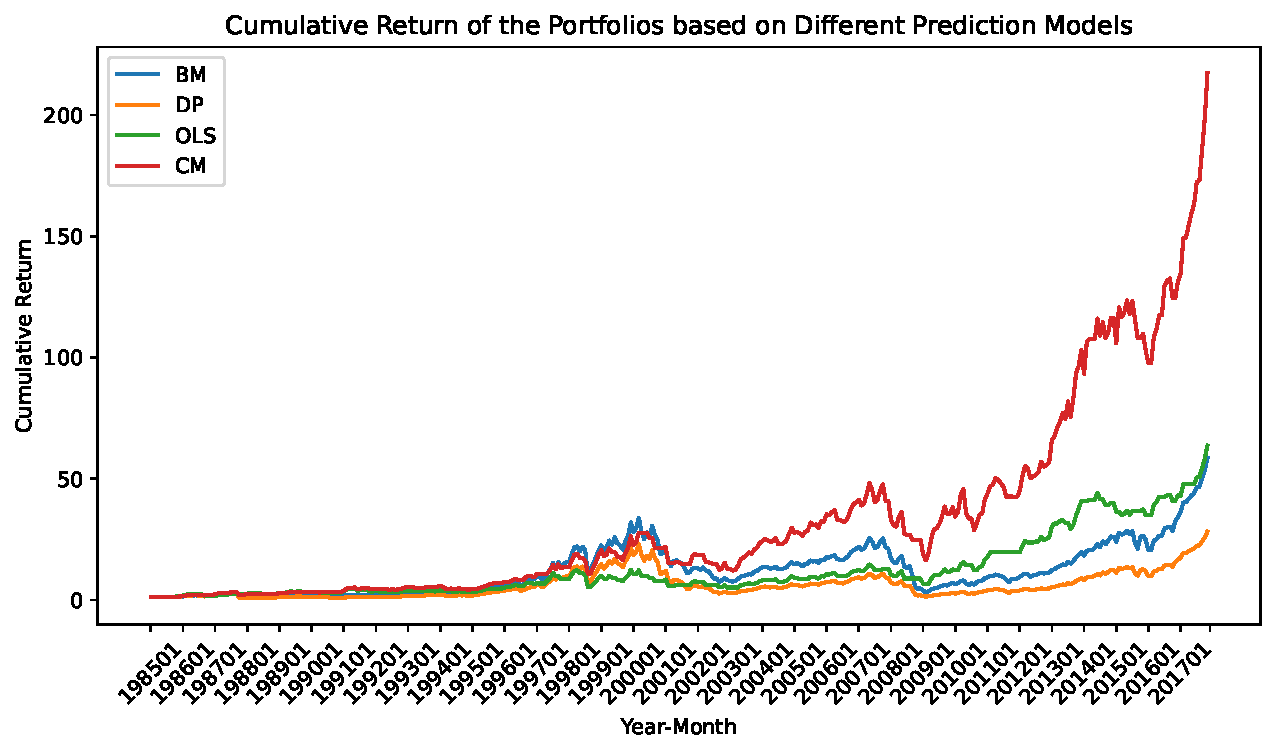
\includegraphics[width=0.85\textwidth]{Out/Ex4_C.pdf}
        \caption{Cumulative returns of the portfolios}
    \end{figure}

    \begin{lstlisting}[language=Python, caption=Python code for portfolio weights, label={lst:q1a}, escapechar=|, frame=single, basicstyle=\small, showstringspaces=false, captionpos=b, breaklines=true, showspaces=false, showtabs=false, keywordstyle=\color{blue}, commentstyle=\color{gray}]
    prediction_data['rolling_var'] = prediction_data.ExcessRet.rolling(60).var()
    gamma = 2
    for prediction_model in ['BM',"DP", "OLS", "CM"]:
        prediction_data['omega_hat'] = prediction_data[prediction_model]/prediction_data['rolling_var']/gamma
        prediction_data['omega_hat_'+prediction_model] = prediction_data['omega_hat']
        prediction_data.loc[prediction_data.omega_hat >= 2,'omega_hat_'+prediction_model] = 2
        prediction_data.loc[prediction_data.omega_hat <= -1,'omega_hat_'+prediction_model] = -1
        prediction_data['r_p_'+prediction_model] = prediction_data['ExcessRet'] + prediction_data['omega_hat_'+prediction_model]*prediction_data['ExcessRet']
    \end{lstlisting}

    \item Now we want to plot the optimal weights of the portfolios. The optimal weights are calculated as mentioned before. The optimal weights of the portfolios are shown in following Figure. We can see that the optimal weights of the portfolios based on the OLS and CM models are not stable and they change over time. However, the optimal weights of the portfolio based on the BM and DP  are stable and they do not change over time. It is interesting to see that the weights from the DP model and the BM model are highly correlated. 
    \begin{figure}[htbp!]
        \centering
        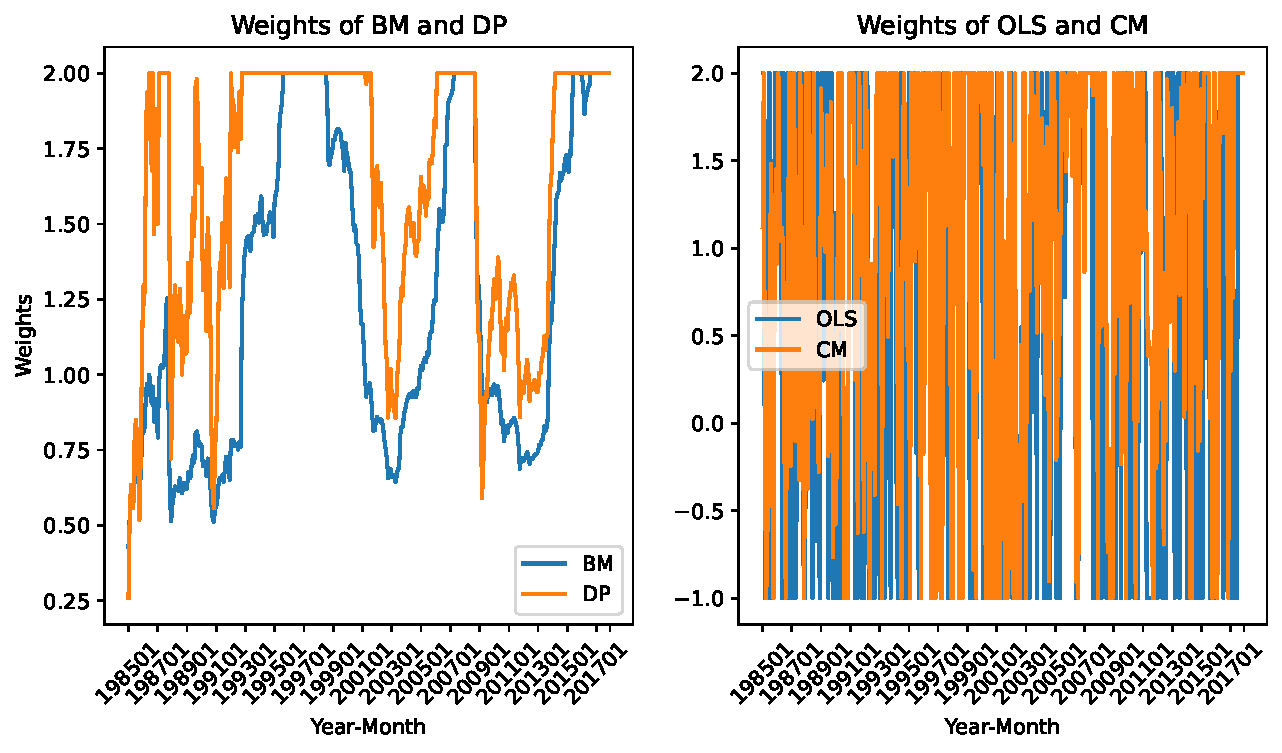
\includegraphics[width=0.85\textwidth]{Out/Ex4_D.pdf}
        \caption{Optimal weights of the portfolios}
    \end{figure}

    \item Now we define a utility function for the investor as:
    \begin{equation*}
        U(\hat{R}_{p,t}^j) = \hat{E}\left[\hat{R}_{p,t}^j\right] - \frac{\gamma}{2} \hat{Var}\left(\hat{R}_{p,t}^j\right)
    \end{equation*}
    and we want to compare the utility of the portfolios based on the predicted excess returns of each model with the utility of the benchmark which is the historical mean. The utility gain is defined as:
    \begin{equation*}
        UG = U(\hat{R}_{p,t}^j) - U(\hat{R}_{p,t}^{BM})
    \end{equation*}
    
    The utility gain for each model is shown in the following table. We can see that the utility gain for the DP model is negative which means that the utility of the portfolio based on the DP model is less than the utility of the benchmark. However, the utility gain for the OLS and CM models are positive which means that the utility of the portfolios based on these models are higher than the utility of the benchmark.

    In this comparison,  we can see that the utility gain for the CM model is the highest which means that the portfolio based on the CM model is the best portfolio among the other portfolios.

    \begin{table}[htbp]
        \centering
        \begin{tabular}{c|c}
            Model & $UG$ \\
            \hline
            DP & -0.003 \\
            OLS & 0.0013 \\
            CM & 0.0043 \\
        \end{tabular}
        \caption{Utility gain for each model}
    \end{table}


\end{enumerate}

\end{document}
